\chapter{Design Implementation}

\section{Overview}

Figure \ref{software_overview.pdf} shows a high level block diagram of the software design.


\section{Server Program}

\subsection{Threads}

The Server Program runs as a multithreaded process under a POSIX compliant GNU/Linux operating system\footnote{Tested on Debian and Ubuntu}. Each thread runs in parallel and is dedicated to a particular task; all threads share the same memory and rescources. The three types of threads we have implemented are:
\begin{enumerate}
  \item Main Thread\ref{} - A single thread which accepts and responds to HTTP requests passed to the program by the HTTP server
  \item Sensor Thread\ref{} - Each sensor in the system is monitored by a single thread
  \item Actuator Thread\ref{} - Each actuator in the system is controlled by a single thread
\end{enumerate}

In reality, threads do not run simultaneously; the operating system is responsible for sharing execution time between threads in the same way as it shares execution times between processes. Because the linux kernel is not deterministic, it is not possible to predict when a given thread is actually running. This renders it impossible to maintain a consistent sampling rate, and necessitates the use of time stamps whenever a data point is recorded.

Figure \ref{} shows a distribution of times between samples for a test sensor with the software sampling as fast as possible. 
Figure \ref{} shows the distribution when the sampling rate is set to 20Hz. Caution should be taken when interpreting these results, as they rely on the accuracy of timestamps recorded by the same software that is being time sliced by the operating system.


RTLinux is a version of the linux kernel that attempts to increase the predictability of when a process will have control\cite{rtlinux}. It was not possible to obtain a real time linux kernel for the BeagleBone. However, testing on an amd64 laptop showed very little difference in the sampling time distribution when the real time linux kernel was used.



\subsection{Safety Mechanisms}



\subsection{Sensors}

Figure \ref{sensor_thread.pdf} shows a flow chart for the thread controlling an individual sensor. This process is implemented by \verb/Sensor_Loop/ and associated helper functions.

All sensors are treated as returning a single floating point number when read. A \verb/DataPoint/ consists of a time stamp and the sensor value. \verb/DataPoint/s are continously saved to a file as long as the experiment is in process. An appropriate HTTP request (see section\ref{}) will cause the main thread of the server program to respond with \verb/DataPoint/s read back from the file. By using independent threads for reading data and transferring it to the GUI, the system does not rely on maintaining a consistent and synchronised network connection. This means that a user can safely close the GUI or even shutdown their computer and return to the experiment later without losing any data.



As the chart indicates, the processes of actually controlling sensor hardware has been abstracted out of the control loop. A \verb/Sensor/ structure is defined in \verb/sensor.h/ to represent a single sensor. When this structure is initialised, function pointers must be provided; these functions can then be called by \verb/Sensor_Loop/ as needed. All functions related to control over specific sensor hardware can be found in the files within the \verb/sensors/ sub directory.

Earlier versions of the software instead used a \verb/switch/ statement based on the \verb/Sensor/'s id number to determine how to obtain the sensor value. This was found to be difficult to maintain as the number and types of sensors supported by the software were increased.



\subsection{Actuators}

Actuators are controlled by threads in a similar way to sensors. Figure \ref{actuator_thread.pdf} shows a flow chart for these threads. This is implemented in \verb/Actuator_Loop/. Control over real hardware is seperated from the main logic in the same way as sensors (relevant files are in the \verb/actuators/ sub directory). The use of threads to control actuators gives similar advantages in terms of eliminating the need to syncronise the GUI and server software.

The actuator thread has been designed for flexibility in how exactly an actuator is controlled. Rather than specifying a single value, the main thread initialises a structure that determines the behaviour of the actuator over a period of time. The current structure represents a simple set of discrete linear changes in the actuator value. This means that a user does not need to specify every single value for the actuator. The Actuator thread stores a value every time the actuator is changed to make it easy to compare the user settings



\subsection{Data Storage and Retrieval}

Each sensor or actuator thread stores data points in a seperate binary file identified by the name of the device. When the main thread receives an appropriate HTTP request, it will read data back from the binary file. To allow for selection of a range of data points from the file, a binary search has been implemented.

Several alternate means of data storage were considered for this project. Binary files were chosen because of the significant performance benefit (see Figure \ref{}) and ease with which data can be read from any location in file and converted directly into values. A downside of using binary files is that the server software must always be running in order to convert the data into a human readable format.

\subsection{Authentication}

The \verb/Login_Handler/ function is called in the main thread when a HTTP request for authentication is received. This function checks the user's credentials and will give them access to the system if they are valid.

Whilst we had originally planned to include only a single username and password, changing client requirements forced us to investigate many alternative authentication methods to cope with multiple users.

Several authentication methods are supported by the server; the method to use can be specified as an argument when the server is started.
\begin{enumerate}
  \item Unix style authentication
  Unix like operating systems store a plain text file (/etc/shadow) of usernames and encrypted passwords. To check a password is valid, it is encrypted and then compared to the stored encrypted password. The actual password is never stored anywhere. The /etc/shadow file must be maintained by shell commands on the beaglebone.

  \item Lightweight Directory Access Protocol (LDAP)
  LDAP is a widely used data base for storing user information. A program that uses LDAP for authentication can query an LDAP server over a network; the LDAP server will respond indicating if the user and password match those stored in its database.

  The UWA user management system (pheme) employs an LDAP server for storing user information and passwords. The software has been designed so that it can interface with an LDAP server configured similarly to the server on UWA's network. Unfortunately we were unable to gain permission to query this server.

  \item MySQL Database
  BLARGH

  MySQL databases are vulnerable to many different security issues. Care should be taken to ensure that all these issues are addressed before deploying the system.
\end{enumerate}

\subsection{Server API}

\subsection{Performance}

Figure \ref{} shows the CPU and memory usage of the server program with different numbers of dummy sensor threads. This gives an idea of how well the system would scale if all sensors were run on the same BeagleBone.

\pagebreak
\begin{figure}[H]
	\centering
	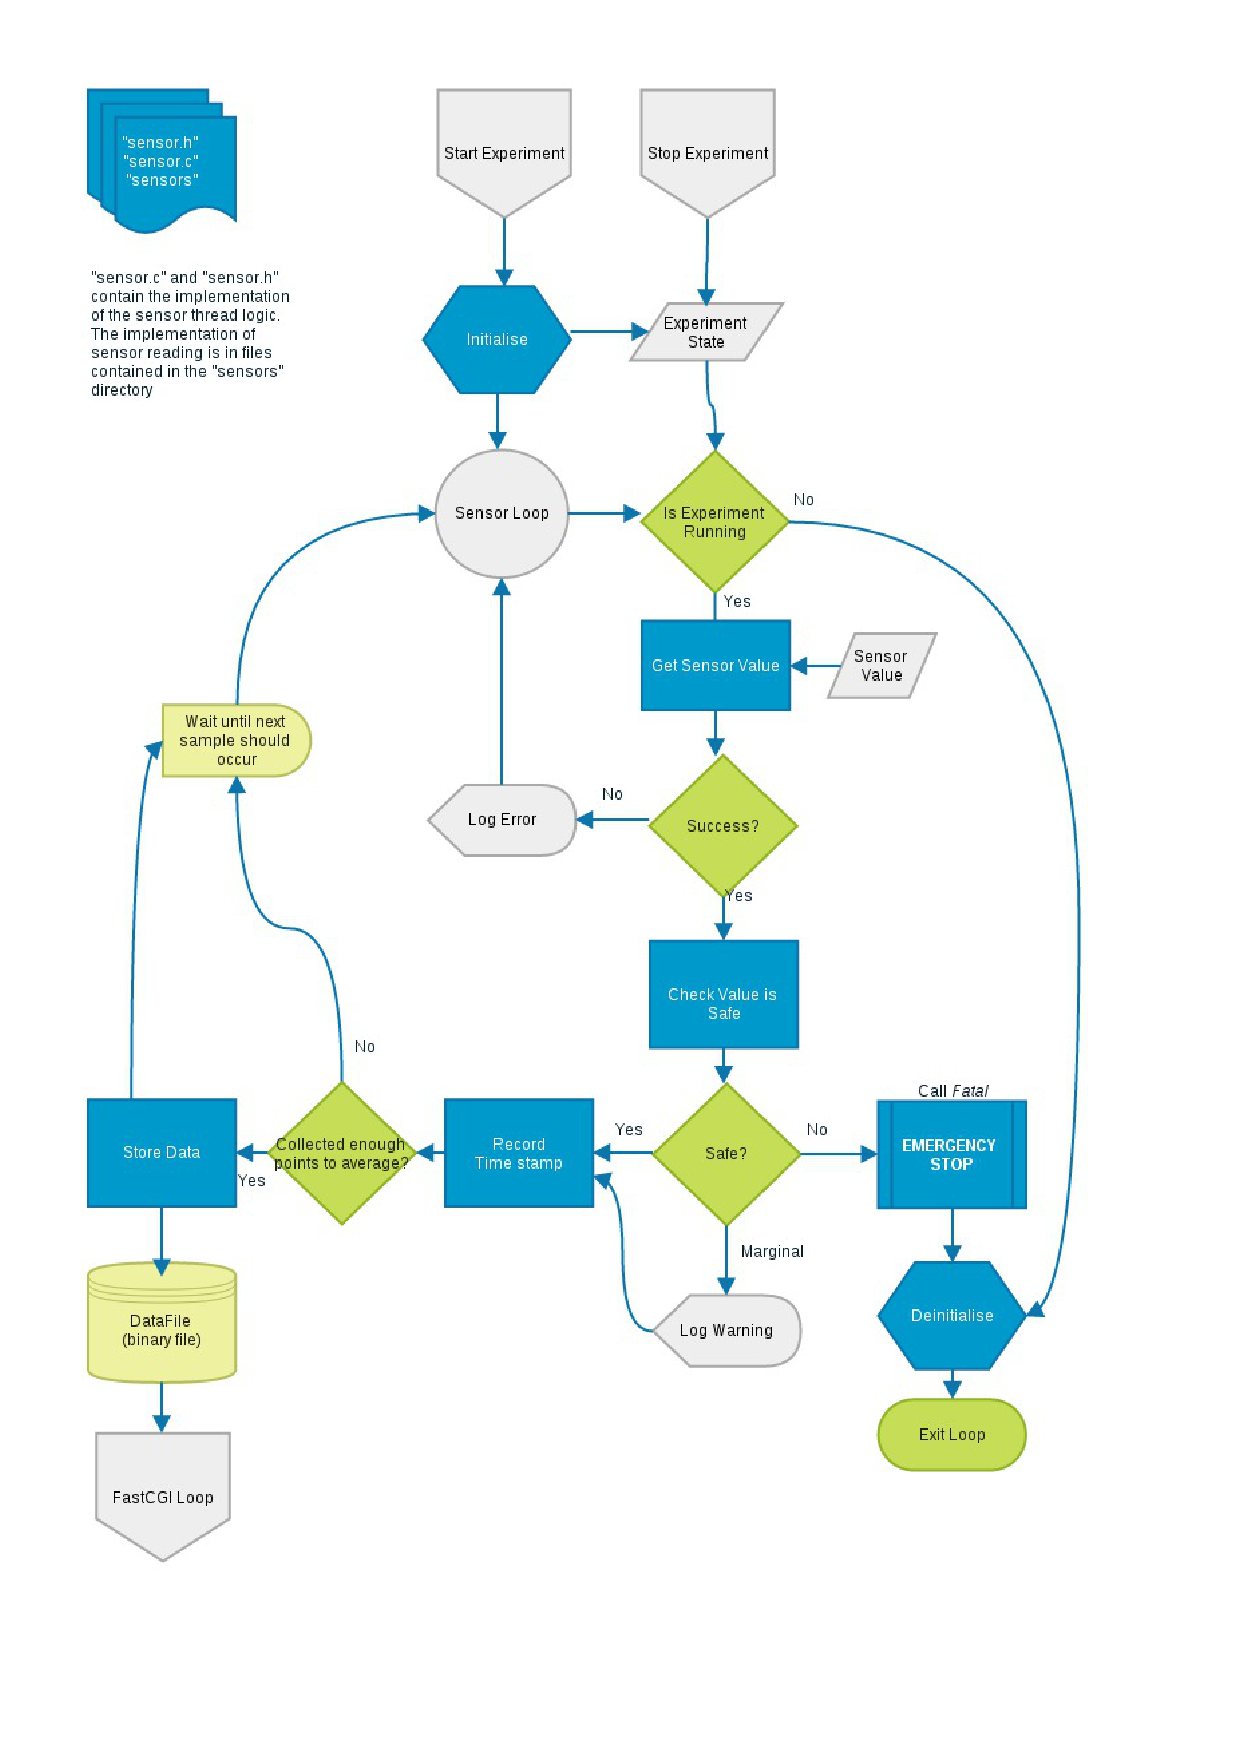
\includegraphics[width=1.1\textwidth]{figures/sensor_thread.pdf}
	\caption{Flow chart for a sensor thread} 
	\label{sensor_thread.pdf}
\end{figure}
\pagebreak
\pagebreak
\begin{figure}[H]
	\centering
	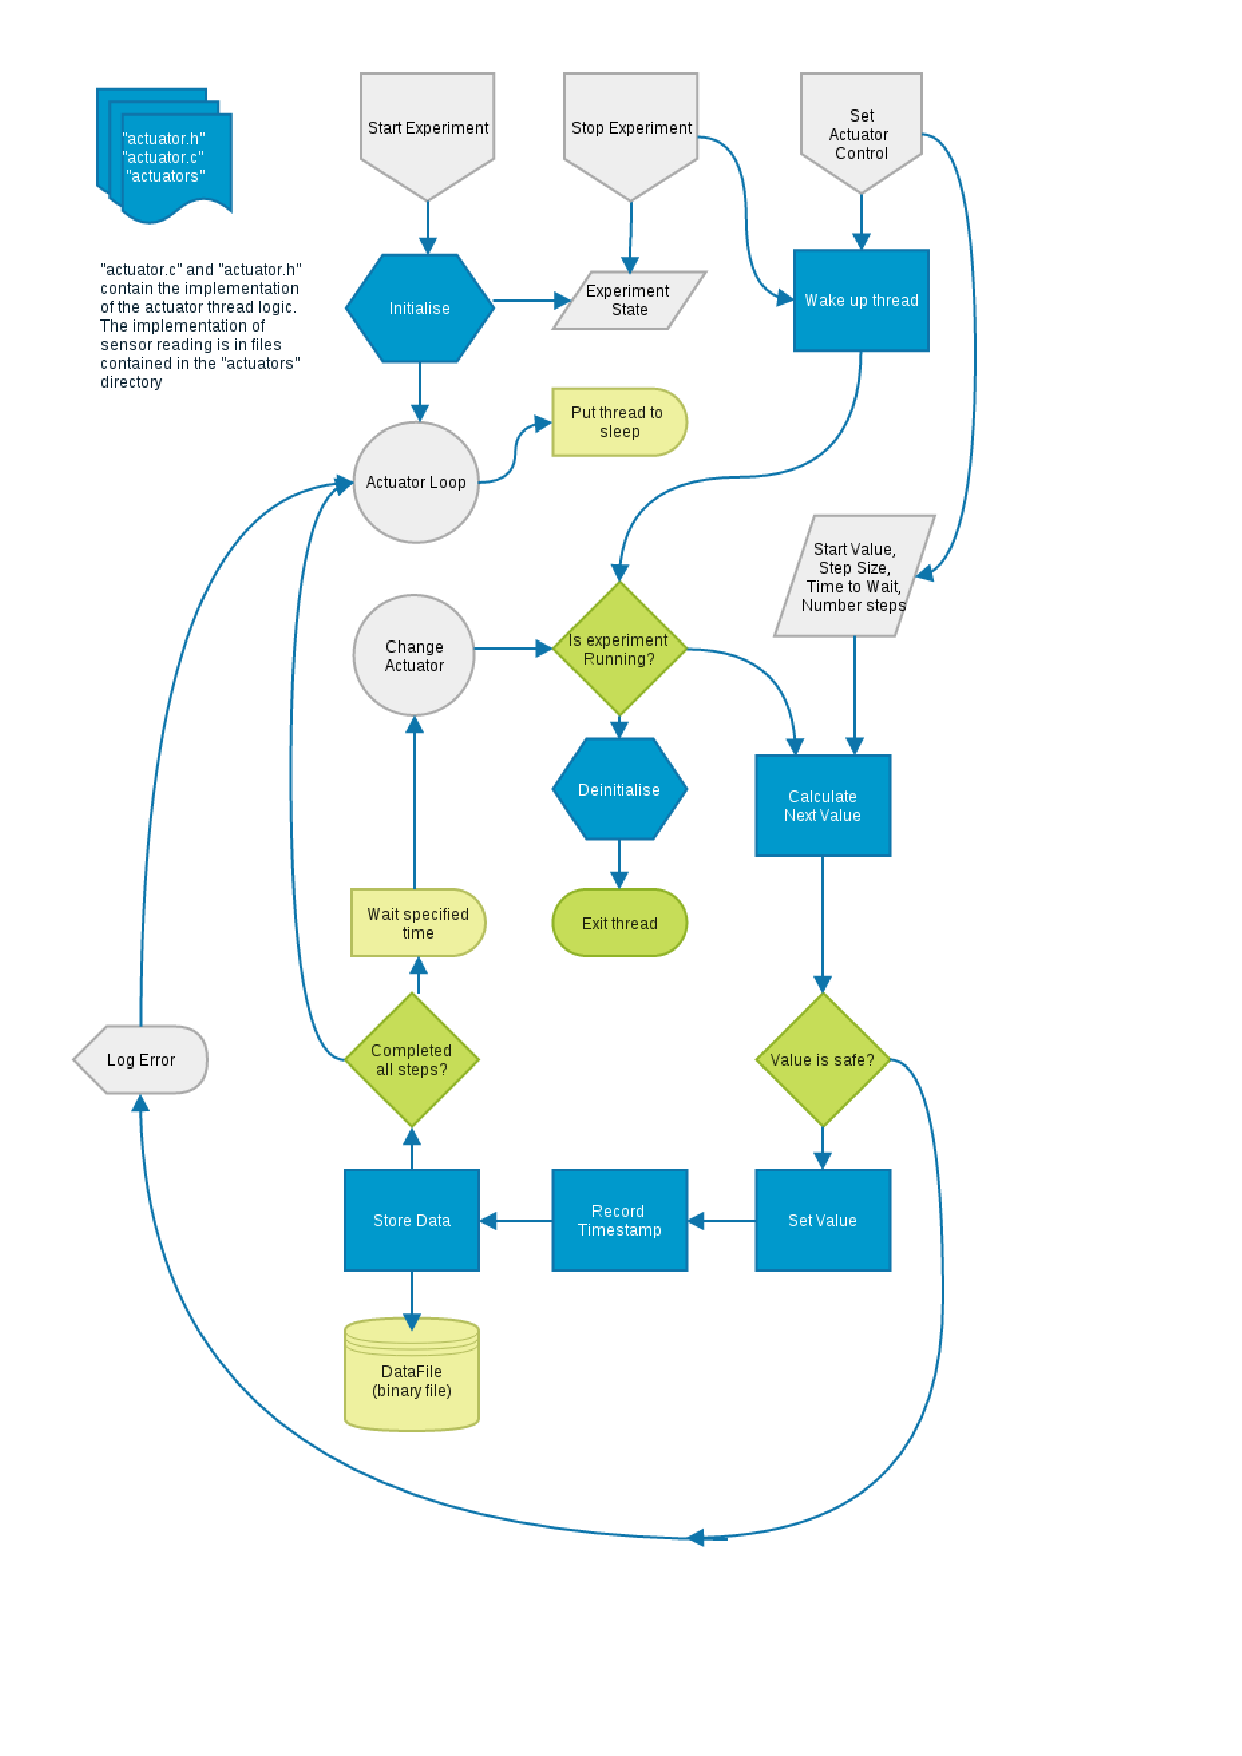
\includegraphics[width=1.1\textwidth]{figures/actuator_thread.pdf}
	\caption{Flow chart for an actuator thread} 
	\label{actuator_thread.pdf}
\end{figure}
\pagebreak

\section{Image Processing}

\section{Client Program}

\subsection{Human Computer Interaction}

\subsection{Interaction with API}









